%%
%% Author: muhamed
%% 27.10.17
%%

% Preamble
\documentclass[11pt]{article}

% Packages
\usepackage{a4wide}
\usepackage[utf8]{inputenc}
\usepackage[ngerman]{babel}
\usepackage{scrextend}      % Intending
\usepackage{graphicx}


% Document
\begin{document}

    \section{ISO/OIS Referenzmodel vs. TCP/IP-Referenzmodell}
    TCP/IP Referenzmodell besteht mehr oder weniger aus den gleichen Schichten
    wie das ISO/OSI-Referenzmodell, jedoch besteht es lediglich aus vier Schichten,
    da die Schichten 5 und 6 nicht verwendet werden.\\
    Es beruht auf den Vorschlägen ,die bei der Fortentwicklung des ARPANET's
    gemacht wurden.
    Diese Art des Modells ist zeitlich vor dem OSI-Referenzmdell entstanden, weshalb
    auch die ERfahrungen dieses Modells in die OSI-Standardisierung miteingeflossen sind.
    Es bildet die Basis für sämtliche Netzwerke, sowie für das OSI-Modell, wie wir es heute
    kennen. \\\\
    IP tu hierbei nichts anderes, als die Daten, mit bestimmten Ziel und Absender, einfach
    nur zu verschicken. In Kombination mit TCP soll letztendlich gewährleistet werden,
    dass die Daten fehlerfrei ankommen.
    Als Ziele der Architektur wurden bei der Entwicklung definiert:
    \begin{enumerate}

        \item{Unabhängigkeit von der verwendeten Netzwerk-Technologie}

        \item{Unabhängigkeit von der Architektur der Hostrechner. }

        \item{Universelle Verbindungsmöglichkeiten im gesamten Netzwerk. }

        \item{Ende-zu-Ende-Quittungen. }

        \item{Standardisierte Anwendungsprotokolle.}

    \end{enumerate}



    Das TCP/IP-Referenzmodell besteht im Gegensatz zum OSI-Modell aus nur vier Schichten.

    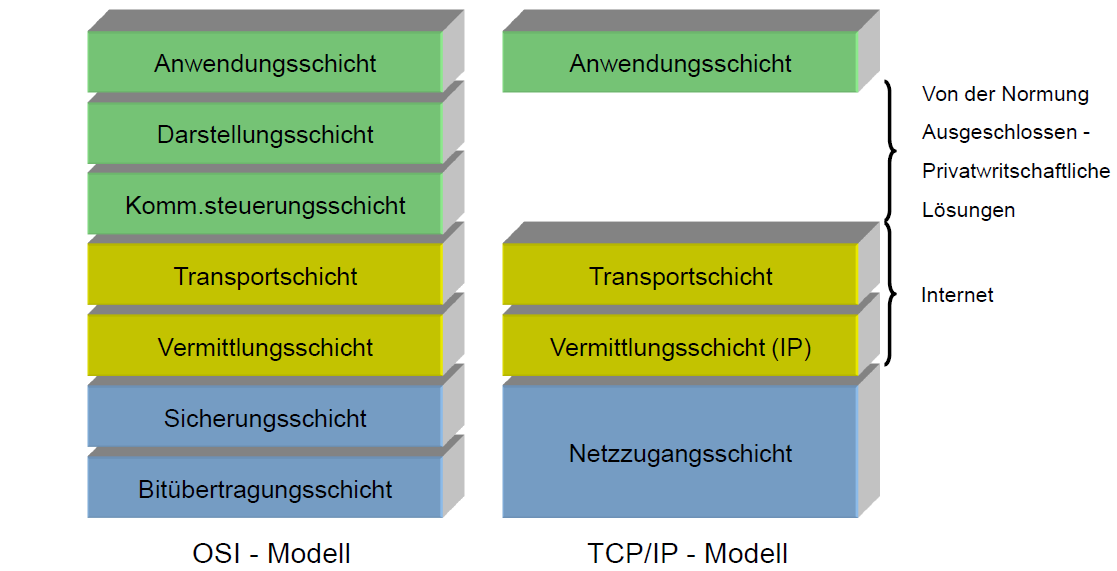
\includegraphics[width = \textwidth]{tcp_ip_model.png}

    % TODO: Search for protocol examples

    \begin{enumerate}

        \item{Application Layer}\\\\
        Umfasst alle höherschichtigen Protokolle des TCP/IP-Modells.
        Zu den ersten Protokollen der Verarbeitungsschicht zählen TELNET (für virtuelle Terminals),
        FTP (Dateitransfer) und SMTP (zur Übertragung von E-Mail).
        Im Laufe der Zeit kamen zu den etablierten Protokollen viele weitere Protokolle wie z.B.
        DNS (Domain Name Service) und HTTP (Hypertext Transfer Protocol) hinzu.


        \item Transport Layer:\\\\
        Ermöglicht wie im OSI-Modell die Kommunikation zwischen Quell- und Zielhost.\\
        Hierzu wurden zwei End-zu-End-Protokolle definiert:\\

        \begin{addmargin}[1em]{1em}

            - Transmisstion Control Protocol (TCP)\\
            \begin{addmargin}[1em]{1em}

                Ist ein zuverlässiges verbindungsorientiertes Protokoll, durch das
                ein Bytestrom fehlerfrei einem anderen Rechner im Internet übermittelt
                werden kann.\\

            \end{addmargin}
            - User Datagram Protocol (UDP)\\
            \begin{addmargin}[1em]{1em}

                UDP ist ein unzuverlässiges Protokoll, welches vorwiegend in Client/Server-
                Umgebungen verwendet wird, in denen es in erster Linie nicht um eine sehr genaue,
                sondern schnelle Datenübertragung geht.\\

            \end{addmargin}
        \end{addmargin}

        \item Internet Layer:\\\\
        Diese Schicht definiert nur ein Protokoll namens IP (Internet Protocol), das alle am Netzwerk
        beteiligten Rechner verstehen kann. Sie hat die Aufgabe IP-Pakete richtig zuzustellen. Dabei
        spielt das Routing der PAkete eine wichtige Rollen. Das Internet Control Message Protocol (ICMP)
        ist fester Bestandteil jedes IP-Implementierung und dient zur Übertragung von Diagnose- und
        Fehlerinformation für das Internet Protocol.\\

        \item Network Layer:\\\\
        Unterhalbe der Internetschicht befindet sich i TCP/IP-Modell eine gro0e Definitionslücke.
        Das Referenzmodell sagt auf dieser Ebene nicht viel aus, was hier passieren soll. Festgelegt ist
        lediglich, dass zur Übermittlung von IP-Paketen ein Host über ein bestimmtes Protokoll an ein Netz
        geschlossen werden muss. Dieses Protokoll ist im TCP/IP-Modell nicht weiter definiert und weicht
        von Netz zu Netz und Host zu Host ab. Dieses Modell macht an dieser Stelle vielmehr Gebrauch von
        bereits vorhandenen PRotokollen, wie z.B. Ethernet (IEE 802.3), Serial Line IP(SLIP), etc.\\
    \end{enumerate}

    TCP Three-Way-Handshake:
    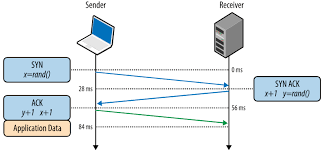
\includegraphics{images.png}

    \begin{enumerate}


        \item Kontakt mit anderem Computer aufnehmen, indem Nachricht x gesendet wird.\\

        \item Nun antwortet der Server mit der Sequenz, die er vom Client bekommen hatte,
        jedoch wurde zu dieser Sequenz plus eins dazu gerechnet.\\

        \item Um Verbindung entgültig aufzubauen, antwortet der Client noch ein letztes mal.\\

    \end{enumerate}

\end{document}